\section{Identificación de requisitos}

La evolución del proyecto obligó a revisar y ampliar los requisitos iniciales a medida que la aplicación dejaba de ser un prototipo centrado exclusivamente en la simulación puntual y pasaba a convertirse en un sistema web más completo, con autenticación, persistencia, progresión pedagógica y despliegue estable.

\subsection{Casos de uso del sistema}

Además de la enumeración textual de requisitos, se elaboraron diagramas de casos de uso para representar de forma visual la interacción entre los actores principales y las funcionalidades del sistema. Estos diagramas permiten separar la visión general del producto de los flujos específicos de autenticación, simulación y progreso educativo.

Debe señalarse que algunos casos de uso secundarios incluidos en los diagramas representan capacidades previstas, de mantenimiento o de evolución del sistema, y no necesariamente flujos completos expuestos en la interfaz final de la versión entregada.

La Figura~\ref{fig:casos-uso-general} ofrece una visión global del sistema, mientras que las Figuras~\ref{fig:casos-uso-autenticacion}, \ref{fig:casos-uso-simulaciones} y \ref{fig:casos-uso-aprendizaje} descomponen los bloques principales asociados al acceso, a la simulación y al progreso pedagógico.

\begin{figure}[htbp]
    \centering
    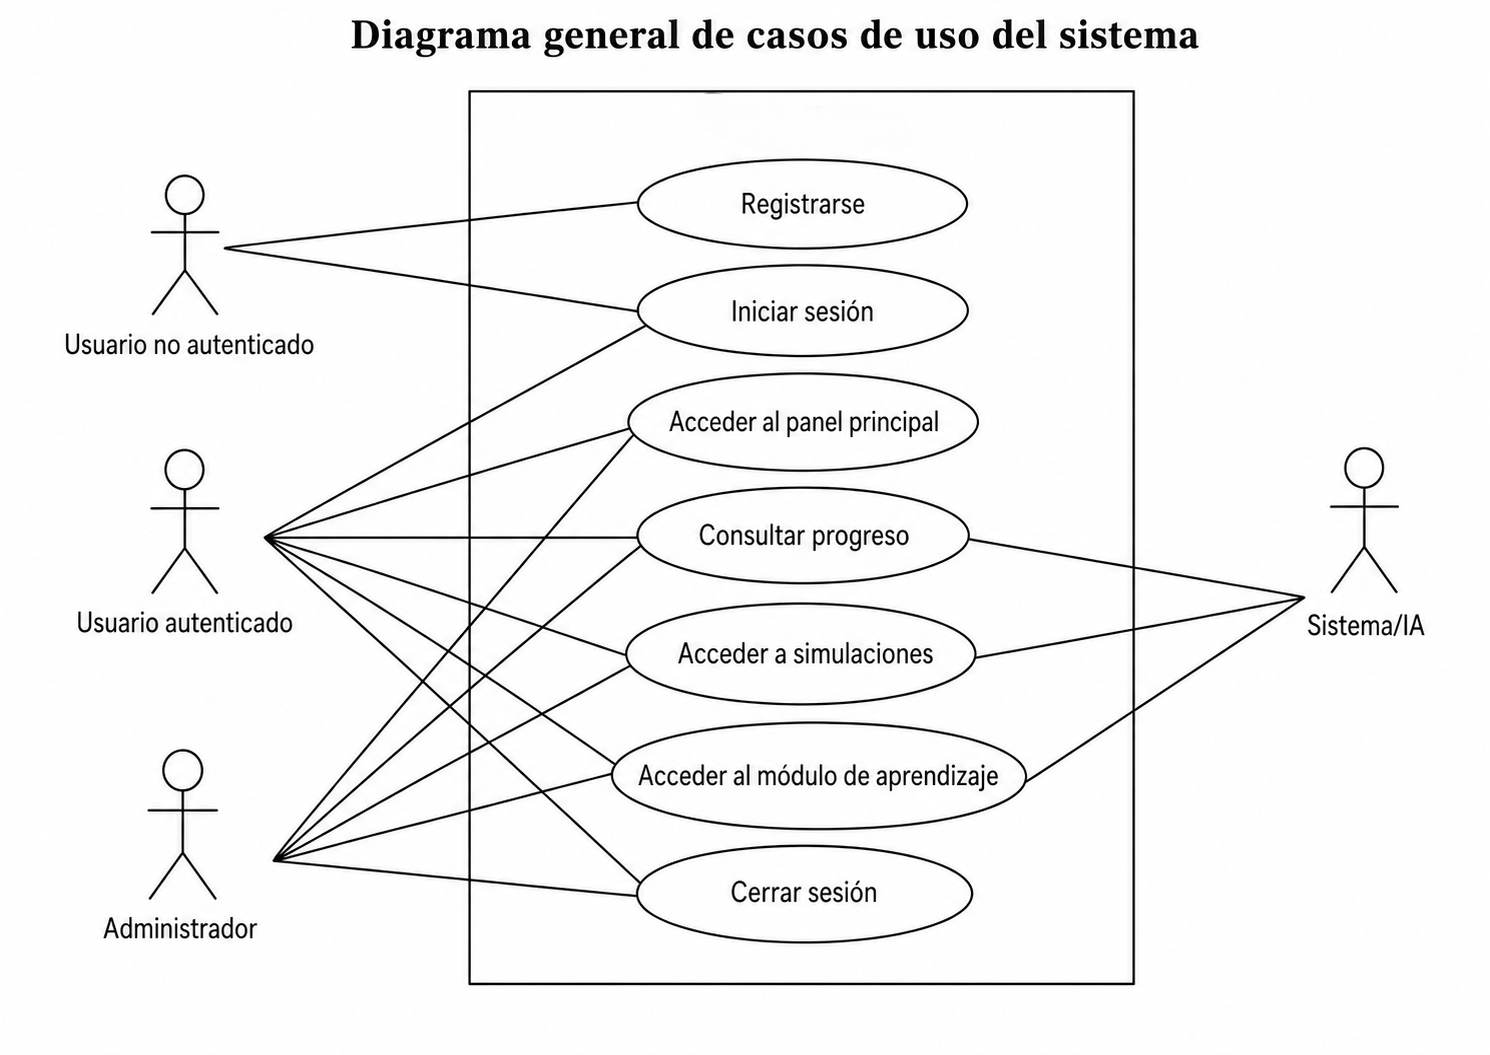
\includegraphics[width=0.92\textwidth]{figs/figura_casos_uso_general.png}
    \caption{Diagrama general de casos de uso del sistema.}
    \label{fig:casos-uso-general}
\end{figure}

\begin{figure}[htbp]
    \centering
    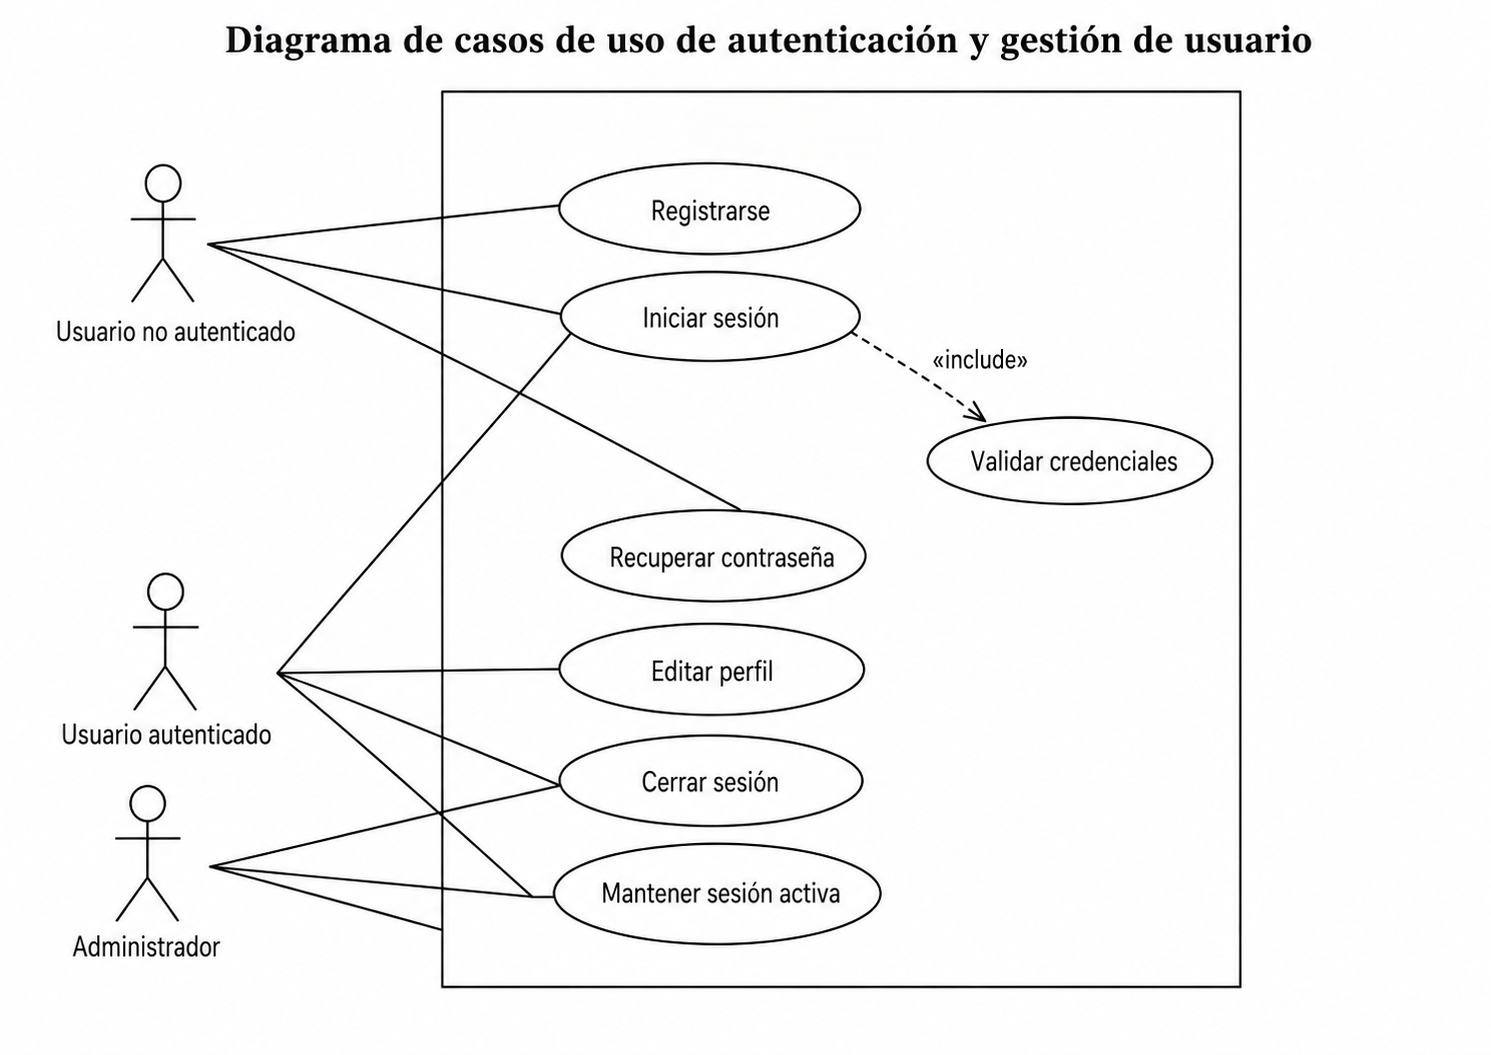
\includegraphics[width=0.9\textwidth]{figs/figura_casos_uso_autenticacion.png}
    \caption{Casos de uso asociados al acceso, autenticación y modo invitado.}
    \label{fig:casos-uso-autenticacion}
\end{figure}

\begin{figure}[htbp]
    \centering
    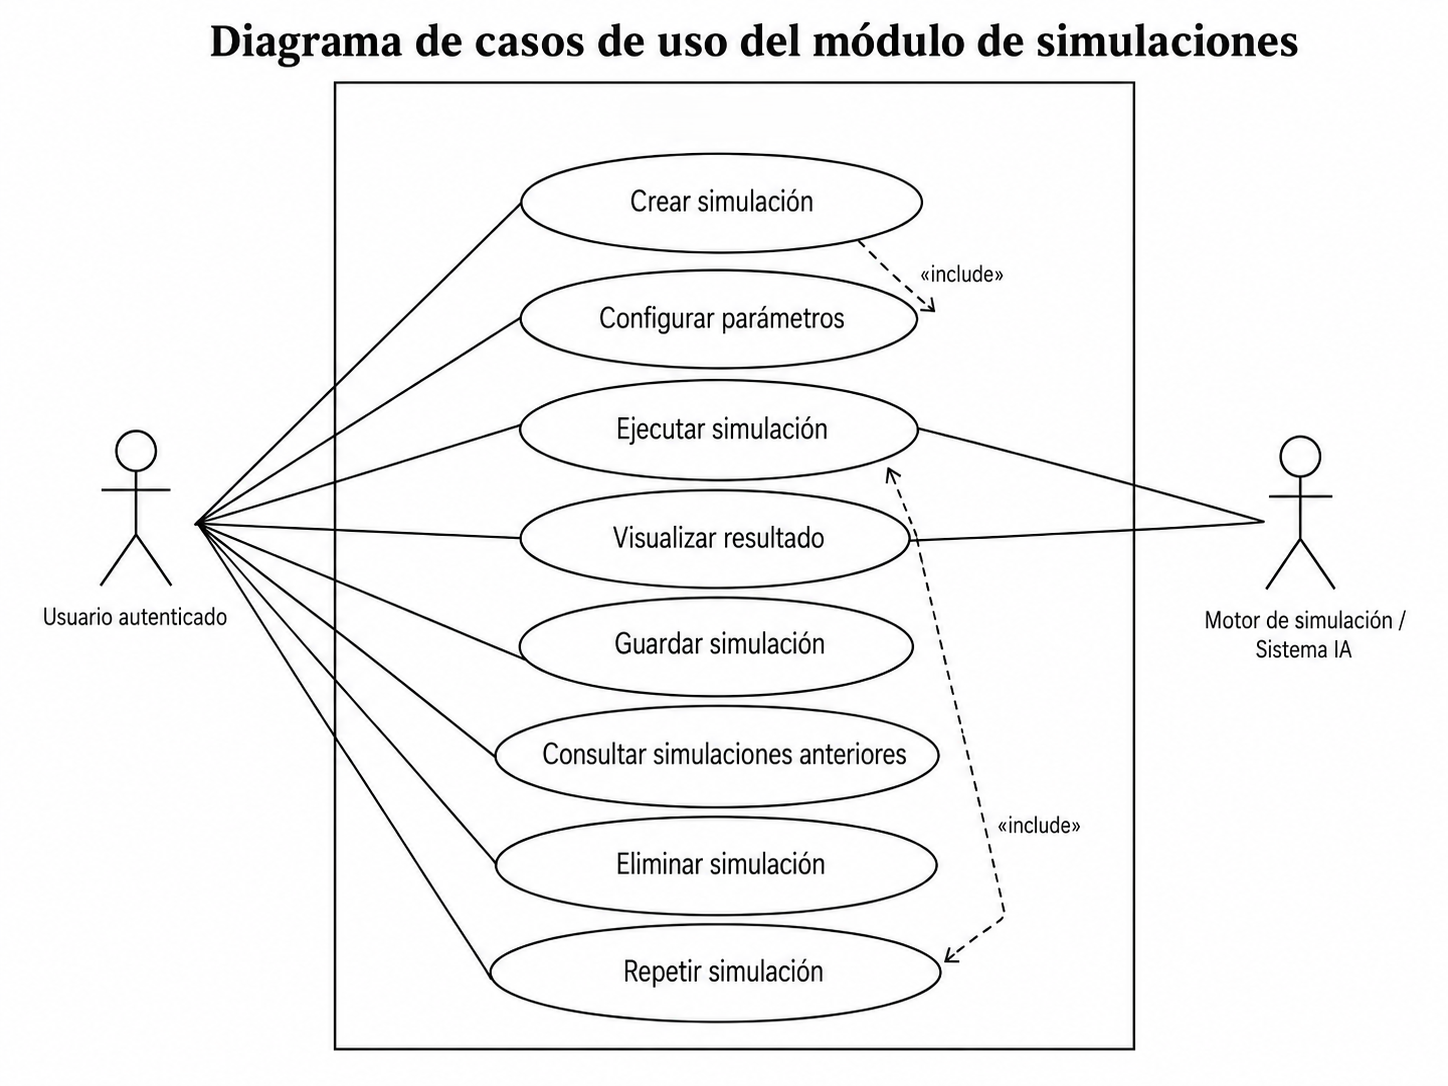
\includegraphics[width=0.92\textwidth]{figs/figura_casos_uso_simulaciones.png}
    \caption{Casos de uso asociados a los módulos de simulación y análisis.}
    \label{fig:casos-uso-simulaciones}
\end{figure}

\begin{figure}[htbp]
    \centering
    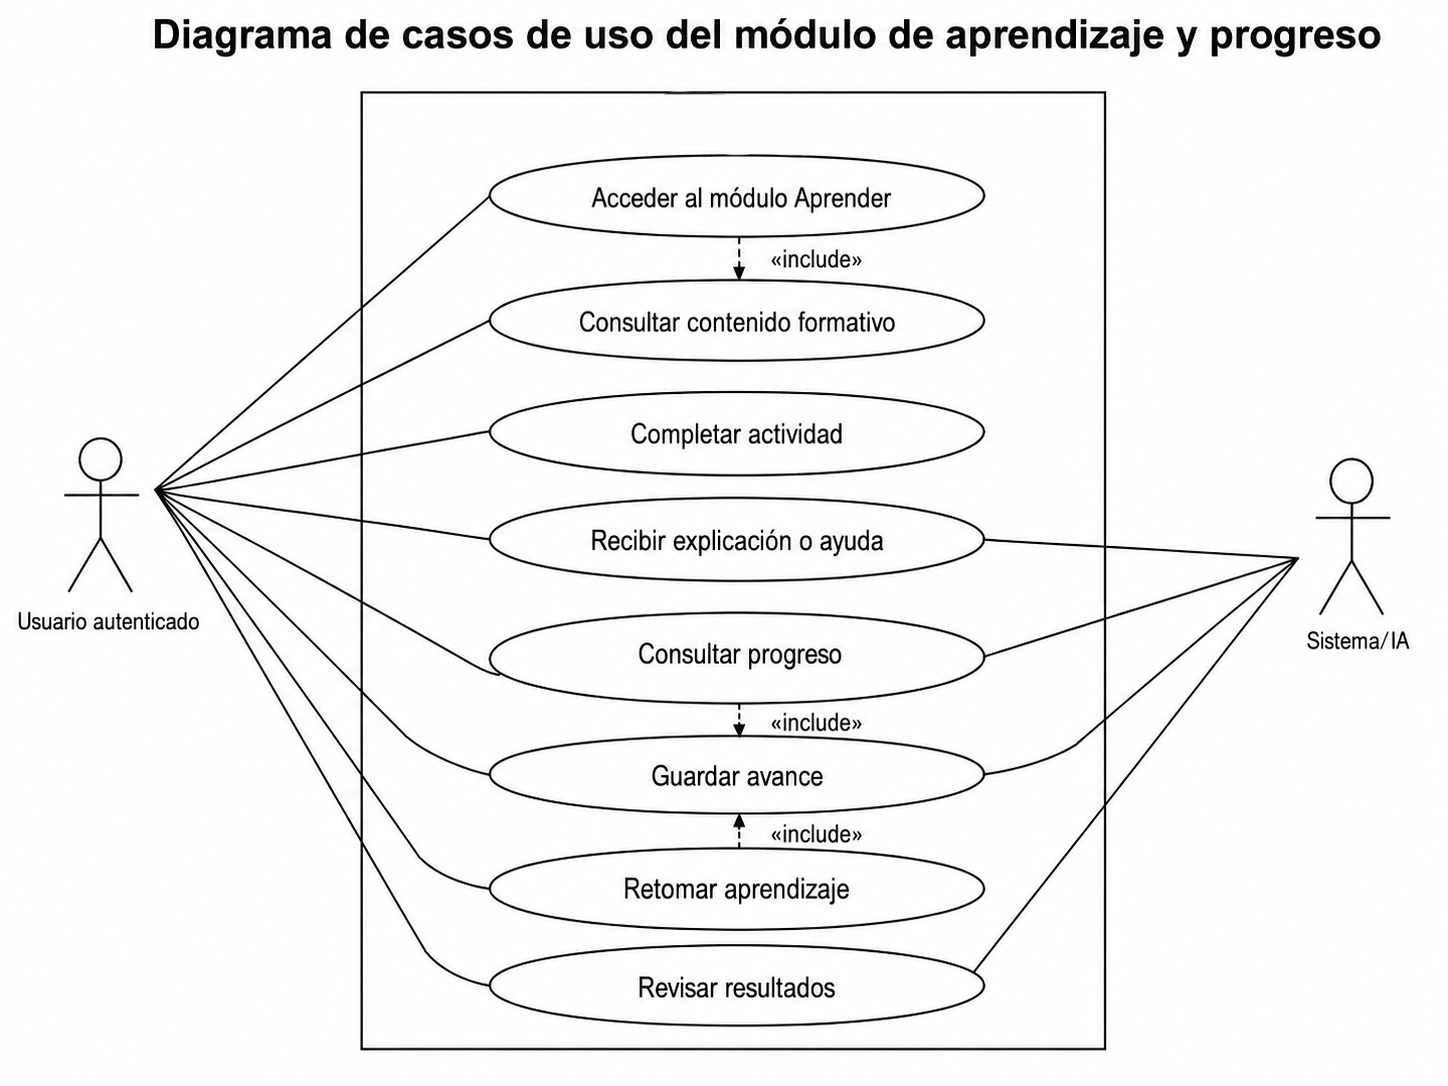
\includegraphics[width=0.92\textwidth]{figs/figura_casos_uso_aprendizaje_progreso.png}
    \caption{Casos de uso asociados al aprendizaje, progreso y apoyo pedagógico.}
    \label{fig:casos-uso-aprendizaje}
\end{figure}

Esta descomposición facilita la trazabilidad entre los requisitos funcionales definidos y los módulos finalmente implementados.

\subsection{Requisitos funcionales}

En su estado final, la aplicación debía satisfacer al menos los siguientes requisitos funcionales:

\begin{itemize}
    \item \textbf{RF-01 Gestión de acceso y perfiles de uso:} el sistema debía diferenciar entre usuario autenticado y usuario invitado, conservando para el primero historial y continuidad, y ofreciendo al segundo una experiencia exploratoria sin persistencia estable.
    \item \textbf{RF-02 Visualización de rentabilidad:} la aplicación debía generar gráficos y métricas comparativas entre cartera, activos individuales y \textit{benchmark}, facilitando la interpretación del resultado histórico.
    \item \textbf{RF-03 Modo Práctica:} el usuario debía poder configurar y ejecutar análisis históricos puntuales sobre activos concretos.
    \item \textbf{RF-04 Modo Carrera:} el sistema debía permitir la gestión de una cartera virtual a lo largo de distintos turnos históricos, con decisiones periódicas, eventos y generación de informe final.
    \item \textbf{RF-05 Readiness quiz:} el acceso al modo carrera debía quedar condicionado por un cuestionario de preparación que reforzase el carácter pedagógico del sistema.
    \item \textbf{RF-06 Modo Horizonte:} la aplicación debía ofrecer un módulo experimental de proyección educativa basado en patrones históricos, dejando explícito que no constituye una predicción real del mercado.
    \item \textbf{RF-07 Tutor IA opcional:} el informe final del modo carrera debía poder complementarse con una capa de análisis educativo asistido por IA, con carácter opcional y sin asesoramiento financiero real.
\end{itemize}

\subsection{Requisitos no funcionales}

A estos requisitos funcionales se sumaron varios requisitos no funcionales determinantes para el cierre del proyecto:

\begin{itemize}
    \item \textbf{RNF-01 Despliegue y disponibilidad:} la aplicación debía desplegarse en Render \cite{render} y mantenerse operativa sobre una infraestructura de bajo coste, asumiendo las limitaciones del plan gratuito.
    \item \textbf{RNF-02 Persistencia real:} la solución debía contar con persistencia fiable mediante PostgreSQL en Render para usuarios, historial y sesiones críticas.
    \item \textbf{RNF-03 Calidad del código:} el desarrollo debía acompañarse de validación técnica repetible mediante \texttt{py\_compile}, \texttt{ruff}, \texttt{black --check} y \texttt{pytest} \cite{pytest,ruff,pep8}.
    \item \textbf{RNF-04 Integración continua:} la rama principal debía quedar respaldada por GitHub Actions \cite{github_actions} como mecanismo de validación automática.
    \item \textbf{RNF-05 Usabilidad y diseño responsive:} la interfaz debía mantener coherencia visual entre pantallas, formularios y estados, tanto en escritorio como en móvil.
\end{itemize}

\section{Metodología de trabajo}

El proceso seguido no fue estrictamente lineal, sino iterativo. A medida que el sistema crecía en complejidad funcional, se adoptó una metodología de trabajo basada en pequeñas iteraciones validadas técnica y visualmente antes de consolidarse.

\subsection{Desarrollo incremental y validación continua}

El proyecto se desarrolló mediante una secuencia de mejoras progresivas sobre funcionalidades existentes. Esta forma de trabajo permitió detectar con rapidez incidencias reales, validar el comportamiento del sistema en producción y refinar el producto sin necesidad de rehacerlo desde cero.

La metodología combinó:
\begin{itemize}
    \item cambios pequeños y trazables;
    \item validación técnica frecuente;
    \item revisión visual en entorno desplegado;
    \item documentación continua de decisiones y resultados.
\end{itemize}

\subsection{Control de versiones y estrategia de ramas}

El control de versiones se apoyó en \textbf{Git} \cite{progit}. La organización final del trabajo distinguió varias ramas con roles claros:

\begin{itemize}
    \item \textbf{main:} rama principal consolidada y versión final oficial del proyecto.
    \item \textbf{bot/render-preview:} rama utilizada para revisión visual en Render durante las fases de rediseño y estabilización.
    \item \textbf{feature/frontend-redesign-v2:} rama de trabajo principal del rediseño frontend por fases.
    \item \textbf{stable/pre-redesign:} rama de congelación funcional previa al rediseño completo.
\end{itemize}

Esta estrategia permitió separar trabajo experimental, validación en preview y consolidación final en \texttt{main}. Como cierre del proceso de rediseño, el repositorio quedó etiquetado con el tag \texttt{v1.1-frontend-redesign}.

\subsection{Apoyo al flujo de trabajo y validación}

Durante la fase final del proyecto se emplearon herramientas de apoyo al flujo de trabajo integradas en la dinámica de documentación, validación y control de versiones, siempre bajo supervisión humana. Su papel se limitó al apoyo en tareas de diagnóstico, organización del trabajo y validación iterativa.

Desde el punto de vista metodológico, este enfoque permitió acelerar tareas repetitivas y mantener trazabilidad sobre ramas, commits y validaciones, sin sustituir en ningún caso la toma de decisiones, la responsabilidad técnica ni la autoría académica del desarrollo.


Con el fin de documentar este aspecto con mayor precisión, se realizó una auditoría del historial Git visible del repositorio principal en el tramo comprendido desde abril de 2026. El resultado mostró \textbf{134 commits} en total durante ese periodo, de los cuales \textbf{131} aparecen firmados por \texttt{OpenClaw Assistant} y \textbf{3} por \texttt{monkeydbot3-del}. Este dato no debe interpretarse como sustitución automática de la autoría intelectual del proyecto, sino como evidencia de un uso intensivo de herramientas asistidas durante la fase de implementación, refactorización controlada, rediseño visual, documentación y validación.

La trazabilidad por ramas y por tipos de trabajo permite distinguir varios bloques metodológicos:

\begin{itemize}
    \item fases iniciales de corrección funcional y mejora incremental del producto;
    \item integración de autenticación, persistencia y endurecimiento del modo carrera;
    \item incorporación de readiness quiz, modo horizonte y Tutor IA;
    \item rediseño frontend iterativo en ramas de preview;
    \item consolidación final en \texttt{main}, hotfixes y documentación de cierre.
\end{itemize}

Desde un punto de vista académico, esta transparencia resulta preferible a minimizar el uso de IA. El criterio seguido en la memoria y en la defensa es reconocer que existió asistencia técnica intensa en el flujo de trabajo, pero que la definición del alcance, la selección de cambios, la validación en entorno real, la integración de resultados, el control de calidad y la responsabilidad final del TFG corresponden al autor.

\section{Planificación temporal y evolución real del proyecto}

Aunque el proyecto partió de una planificación inicial clásica, su evolución efectiva se organizó en hitos funcionales y de estabilización más próximos a un desarrollo iterativo. La Tabla~\ref{tab:hitos_proyecto_final} resume los hitos principales hasta el cierre.

\begin{table}[h]
\centering
\renewcommand{\arraystretch}{1.2}
\begin{tabular}{|p{0.22\textwidth}|p{0.42\textwidth}|p{0.22\textwidth}|}
\hline
\textbf{Hito} & \textbf{Descripción} & \textbf{Resultado} \\ \hline
Modos base del sistema & Construcción del núcleo inicial de análisis y simulación & Base funcional de la aplicación \\ \hline
Autenticación y persistencia & Incorporación de login por correo, modo invitado e historial persistente & Diferenciación real entre perfiles de usuario \\ \hline
Readiness y modo carrera & Integración del cuestionario de preparación y persistencia progresiva de sesiones & Flujo pedagógico y continuidad de juego \\ \hline
Modo Horizonte & Incorporación del módulo experimental no predictivo & Extensión educativa del ecosistema de simulación \\ \hline
Rediseño frontend por fases & Ejecución de siete fases de rediseño visual y revisión global final & Interfaz coherente y más madura \\ \hline
Validación en Render & Revisión del comportamiento real en entorno desplegado & Corrección de problemas visuales y funcionales reales \\ \hline
Consolidación en main & Integración de la versión validada y creación de tag final & Cierre estable del frontend en rama principal \\ \hline
Hotfix final auth/navbar & Corrección del renderizado de estado autenticado en navegación interna & Coherencia final entre sesión real y UI \\ \hline
\end{tabular}
\caption{Hitos principales de la evolución real del proyecto hasta su cierre.}
\label{tab:hitos_proyecto_final}
\end{table}

\subsection{Rediseño frontend por fases}

Una parte sustancial del cierre del proyecto consistió en un rediseño frontend ejecutado por fases. El trabajo no se planteó como una reescritura completa, sino como una secuencia de mejoras controladas sobre la interfaz ya existente.

Las fases principales fueron las siguientes:

\begin{itemize}
    \item Fase 1: sistema visual base.
    \item Fase 2: home, login, registro y navbar.
    \item Fase 3: aprender y readiness quiz.
    \item Fase 4: modo práctica o nuevo análisis.
    \item Fase 5: modo carrera.
    \item Fase 6: modo horizonte.
    \item Fase 7: revisión global final de coherencia visual y responsive.
\end{itemize}

La validación de estas fases se realizó primero sobre la rama de vista previa y después sobre la rama principal, una vez confirmada su estabilidad. El detalle funcional de cada fase se desarrolla en el capítulo de implementación, por lo que aquí solo se recoge su papel dentro de la planificación y de la evolución global del proyecto.

\section{Estudio de viabilidad}

\subsection{Viabilidad técnica}

El proyecto resultó técnicamente viable gracias a la madurez del ecosistema Python, al uso de Flask como \textit{microframework} y a la disponibilidad de servicios de despliegue y base de datos accesibles en la nube. La combinación entre Render y PostgreSQL permitió validar el sistema con un grado de realismo suficiente para el alcance académico del TFG.

\subsection{Viabilidad económica}

Desde el punto de vista económico, el uso de herramientas de código abierto y de planes gratuitos redujo el coste directo de infraestructura. No obstante, la experiencia final también puso de manifiesto la fragilidad de este tipo de servicios cuando expiran recursos asociados, como ocurrió con una base de datos anterior de Render. Por ello, el modelo seguido es viable para un TFG, aunque no necesariamente óptimo como solución estable a largo plazo.

\subsection{Viabilidad legal y de datos}

La aplicación utiliza bibliotecas y herramientas bajo licencias permisivas y se apoya en datos públicos accesibles mediante Yahoo Finance. Sin embargo, al incorporar autenticación y persistencia de usuarios, la dimensión de protección de datos deja de poder describirse como puramente anónima. Aunque el alcance del TFG no persigue explotación comercial ni tratamiento masivo de datos, el sistema final sí distingue entre identidad autenticada e invitada, lo que obliga a considerar con mayor cuidado la gestión responsable de credenciales, sesiones y datos persistidos.

\section{Análisis de riesgos}

Los riesgos identificados durante la evolución real del proyecto fueron los siguientes:

\begin{table}[h]
\centering
\begin{tabular}{|p{0.28\textwidth}|p{0.27\textwidth}|p{0.32\textwidth}|}
\hline
\textbf{Riesgo} & \textbf{Impacto} & \textbf{Mitigación aplicada} \\ \hline
Cambios o límites del proveedor de datos & Alto & Tratamiento controlado de errores, reintentos y degradación amistosa ante incidencias externas. \\ \hline
Expiración o fragilidad de infraestructura gratuita & Medio/alto & Recreación de base de datos en Render y revalidación funcional del sistema sobre la nueva instancia. \\ \hline
Regresiones tras cambios iterativos & Alto & Validación frecuente con \texttt{py\_compile}, \texttt{ruff}, \texttt{black}, \texttt{pytest} y GitHub Actions. \\ \hline
Incoherencias visuales entre pantallas & Medio & Trabajo por fases de rediseño y revisión en Render antes de consolidar en \texttt{main}. \\ \hline
Errores de sesión o navegación en producción & Medio & Detección de incidencias reales y aplicación de hotfixes específicos, como la corrección final del estado de navbar. \\ \hline
\end{tabular}
\caption{Riesgos principales detectados y mecanismos de mitigación aplicados.}
\label{tab:riesgos_actualizados}
\end{table}
